\documentclass{article}
\usepackage{tikz}
\usepackage{adjustbox}

\begin{document}

% \begin{center}
%     {\ttfamily \textbf{UNITED STATES}} \\
%     {\ttfamily \textbf{AIR STATUS DISPLAY}}
% \end{center}

\vspace{1em}


\begin{adjustbox}{left}
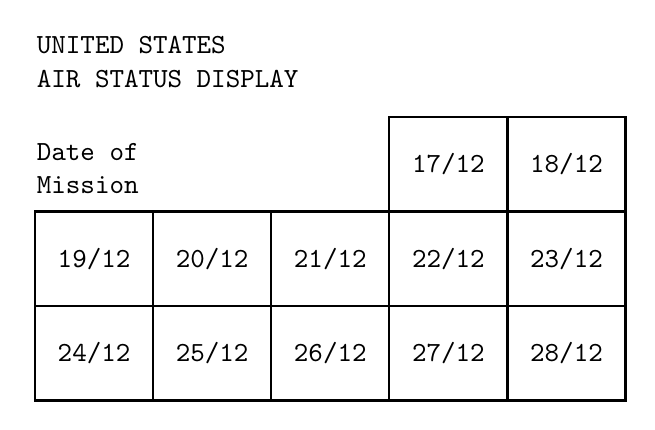
\begin{tikzpicture}
    % Let's move the UNITED STATES text above to a node in the tikz
    % picture, align it to the left and move it up a bit
    \node[anchor=west, align=left] at (-0.1, 0.7) {%
        \ttfamily\textbf{UNITED STATES} \\
        \ttfamily \textbf{AIR STATUS DISPLAY}%
    };

    \node[anchor=west, align=left] at (-0.1, -0.65) {%
        \ttfamily\textbf{Date of} \\
        \ttfamily\textbf{Mission}%
    };

    % Define box size
    \def\boxwidth{1.5}
    \def\boxheight{1.2}

    \foreach \x [count=\i] in {17, 18} {
        \pgfmathsetmacro\xpos{\i + 2}
        \draw[thick] (\xpos*\boxwidth, 0) rectangle (\xpos*\boxwidth + \boxwidth, -\boxheight);
        \node at (\xpos*\boxwidth + 0.75, -0.6) {\ttfamily \textbf{\x/12}};
    }

    % Second row (middle row)
    \foreach \x [count=\i] in {19, 20, 21, 22, 23} {
        \pgfmathsetmacro\xpos{\i - 1}
        \draw[thick] (\xpos*\boxwidth, -\boxheight) rectangle (\xpos*\boxwidth + \boxwidth, -2*\boxheight);
        \node at (\xpos*\boxwidth + 0.75, -1.8) {\ttfamily \textbf{\x/12}};
    }

    % Third row (bottom row)
    \foreach \x [count=\i] in {24, 25, 26, 27, 28} {
        \pgfmathsetmacro\xpos{\i - 1}
        \draw[thick] (\xpos*\boxwidth, -2*\boxheight) rectangle (\xpos*\boxwidth + \boxwidth, -3*\boxheight);
        \node at (\xpos*\boxwidth + 0.75, -3.0) {\ttfamily \textbf{\x/12}};
    }

\end{tikzpicture}
\end{adjustbox}

\end{document}
